\section{Aufgabenblatt 4}

\subsection{Error Handling}
	Eigentlich sollte sich PBS darum kümmern Jobs zu verschieben und 
	neuzustarten, wenn ein Knoten abstürzt auf dem ein Job lief.

	Da sich einzelnen Jobs und ihr Zustand schlecht überwachen lassen,
	verwenden wir folgenden Ansatz.
	Wir messen die Zeit die 42\% der der Jobs benötigen.
	Sind soviele Jobs fertig und ist die Zeit dieser Jobs um mehr als das
	doppelte überschritten, werden die restlichen Jobs neu gestartet.

	Bei Speichermangel wird der Nutzer gefragt,
	ob entweder alle bsi jetzt berechneten Zwischenergebnisse gelöscht und
	das Skript beendet werden sollen oder ob alle Jobs angehalten werden sollen.
	In diesem Fall werden alle unfertigen Jobs angehalten.
	Ist wieder genug Speicherplatz vorhanden,
	können die Jobs auf die Eingabe des Nutzer fortgesetzt werden.


\subsection{Performanz}

In Tabelle \ref{tab:povrayperformance}  und Abbildung \ref{fig:povrayperfplot} lässt sich der zeitliche Vorteil gut erkennen. 
		So wird deutlich, das durch Verwendung des mehrer Knoten ein Overhead ensteht,
		welcher bis zu einer Bildgröße von etwa 500*500 Pixel erkennbar ist.
		Werden die Bilder größer ist der verteilte Ansatz schneller.
		Bei Bilder mit mehr als 2000*2000 Pixel zeigt sich auch der Vorteil von einer größeren Anzahl Knoten.
	
		\begin{table}[h]
		\begin{center}
		\begin{tabular}{r l l l} 
			\toprule
			Bildgröße	&	1 Knoten		&	10 Knoten	&	20 Knoten	\\
			\midrule
			100*100		&	1.691		&	35.773	&	37.141	\\
			200*200		&	4.943		&	36.063	&	36.91	\\
			300*300		&	10.232	&	36.207	&	37.264	\\
			500*500		&	27.197	&	36.31		&	37.004	\\
			1000*1000	&	106.417	&	36.174	&	37.215	\\
			2000*2000	&	449.276	&	121.691	&	72.73	\\
			4000*4000	&	1700.454	&	404.263	&	228.201	\\
			\bottomrule
		\end{tabular}
		\caption{Übersicht über die Laufzeiten von Povray bei Verwendung mehrere Knoten in Sekunden mit der Datei ``landscape.pov''.}
		\label{tab:povrayperformance}
		\end{center}
		\end{table}
	
		Zu beachten ist das durch das Warten auf den Abschluss der Jobs Verzerrungen aufgetreten seien können,
		da nur all 5 Sekunden überprüft wird ob die Jobs abgeschlossen sind.

		\vspace{2cm}
		\begin{figure}[ht!]
			\begin{center}
				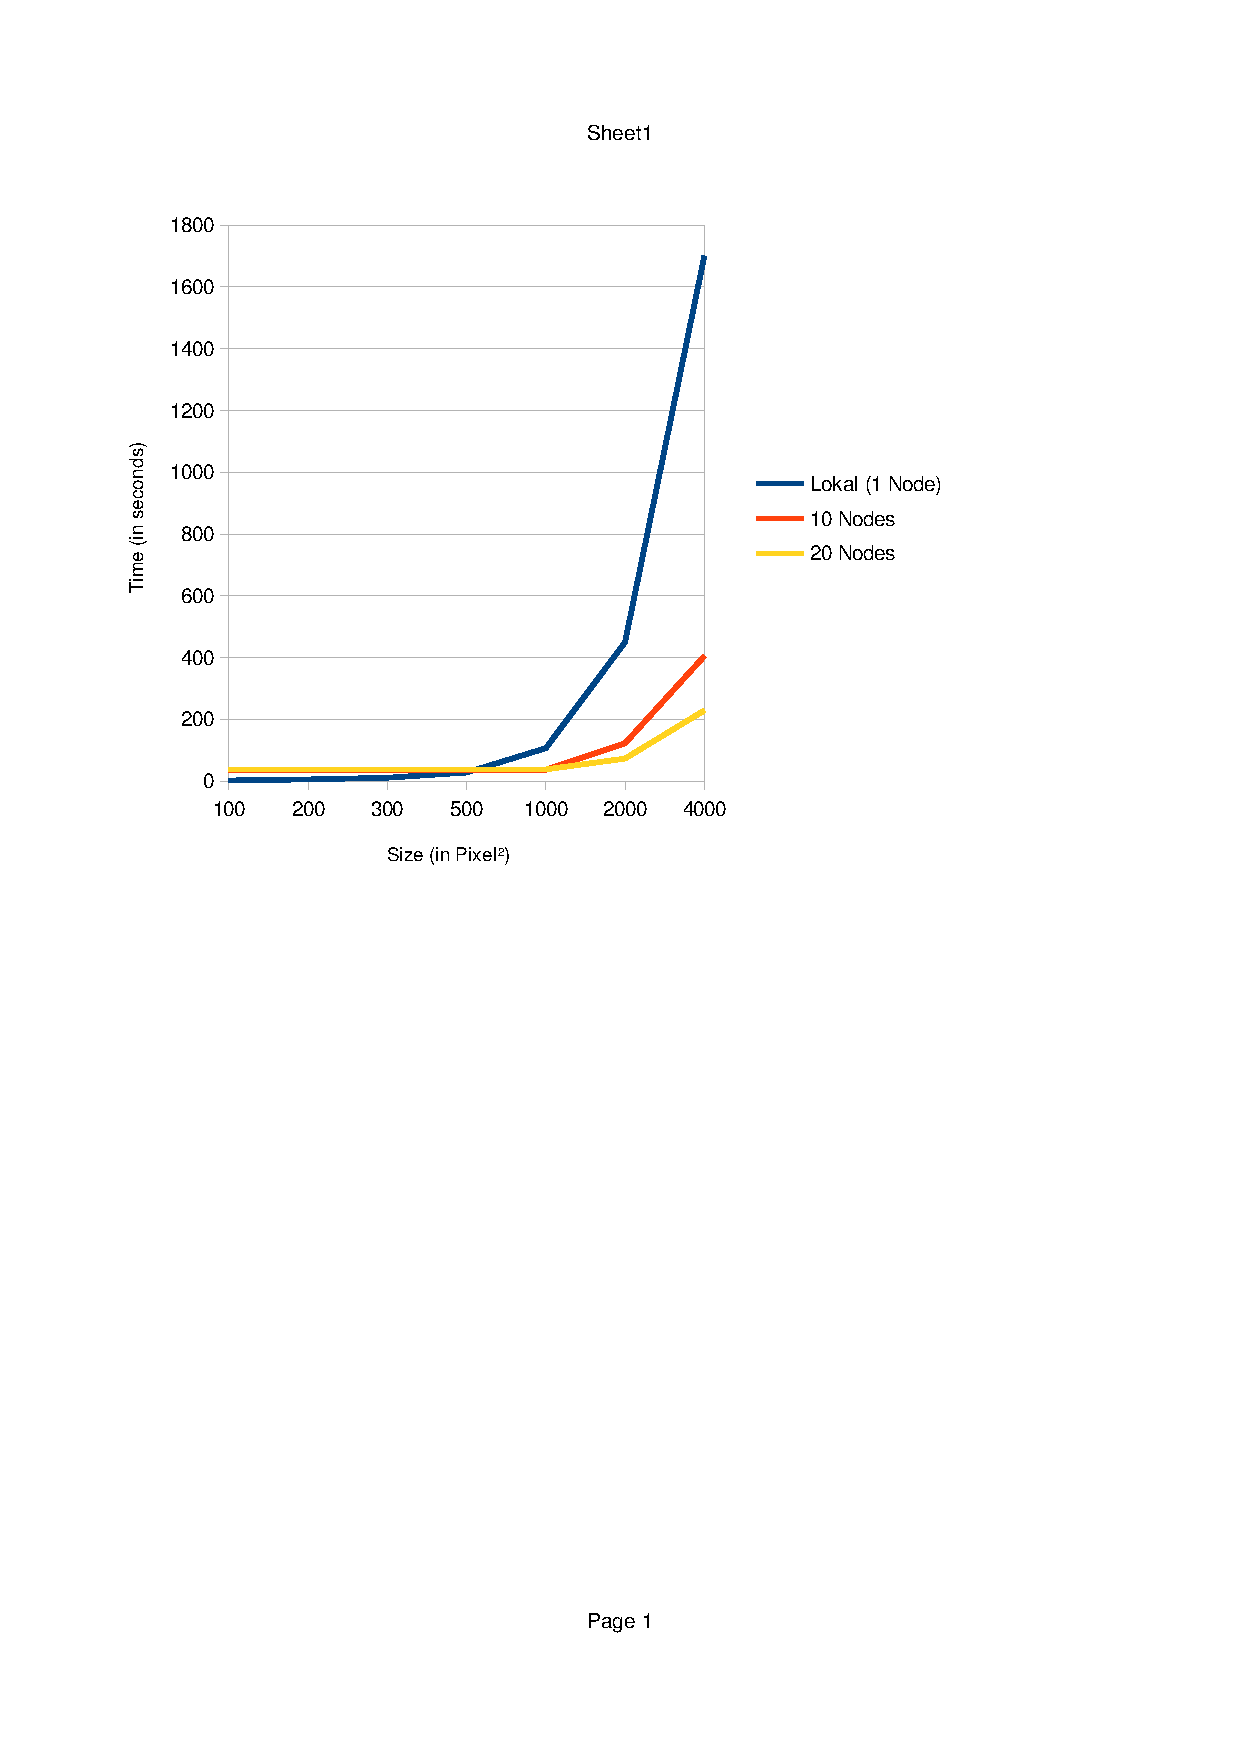
\includegraphics[trim=2cm 14cm 4cm 3cm,clip]{./task_03/plot}
			\end{center}
			\caption{Plot der Performanzauswertung.}
			\label{fig:povrayperfplot}
		\end{figure}
		
	
